%%%%%%%%%%%%%%%%%%%%%%%%%%%%%%%%%%%%%%%%%%%%%%%%%%%%%%%%%%%%%%%%%%%%%%%%%%%
%
% Template for a LaTex article in English.
%
%%%%%%%%%%%%%%%%%%%%%%%%%%%%%%%%%%%%%%%%%%%%%%%%%%%%%%%%%%%%%%%%%%%%%%%%%%%

\documentclass{article}

% AMS packages:
\usepackage{amsmath, amsthm, amsfonts}
\usepackage[margin=2cm]{geometry}% by courtesy of Micro
\usepackage{pgfplots}
\usepackage{tikz}
\usepackage{tcolorbox}
\usetikzlibrary{arrows,shapes.geometric,fit,matrix}
\usetikzlibrary{backgrounds,calc,chains,decorations,positioning}

\tcbset{
    nobeforeafter,
    %colbacktitle=blue!20,
    %colback=yellow!30,
    %coltitle=black,
    %coltext=black,
    %fontupper=\sffamily\bfseries\LARGE,
    %width=.5\linewidth,
}

% Theorems
%-----------------------------------------------------------------
\newtheorem{thm}{Theorem}[section]
\newtheorem{cor}[thm]{Corollary}
\newtheorem{lem}[thm]{Lemma}
\newtheorem{prop}[thm]{Proposition}
\theoremstyle{definition}
\newtheorem{defn}[thm]{Definition}
\theoremstyle{remark}
\newtheorem{rem}[thm]{Remark}

% Shortcuts.
% One can define new commands to shorten frequently used
% constructions. As an example, this defines the R and Z used
% for the real and integer numbers.
%-----------------------------------------------------------------
\def\RR{\mathbb{R}}
\def\ZZ{\mathbb{Z}}

% Similarly, one can define commands that take arguments. In this
% example we define a command for the absolute value.
% -----------------------------------------------------------------
\newcommand{\abs}[1]{\left\vert#1\right\vert}

% Operators
% New operators must defined as such to have them typeset
% correctly. As an example we define the Jacobian:
% -----------------------------------------------------------------
\DeclareMathOperator{\Jac}{Jac}

%-----------------------------------------------------------------
\title{Binary Parallel \LaTeX\ Plot $01$}
\author{Rajdeep Chatterjee\\
  \small School of Computer Engineering\\
  \small KIIT Deemed to be University\\
  \small Bhubaneswar 751024, India
}

\begin{document}
\maketitle

\tikzset{near start abs/.style={xshift=1cm}}

\begin{figure}[!ht]
\centering
\begin{tikzpicture}[node distance=6mm, >=latex',
node distance = 1 cm,
                > = stealth,
      start chain = going below,
every node/.style = {align=center},
 startstop/.style = {rectangle, align=center, rounded corners, draw=red, fill=red!20,
                     minimum width=3cm, minimum height=1cm, font=\large\sffamily},
  decision/.style = {draw=#1, fill=#1!20,
                     diamond, minimum width=3cm, minimum height=1.5cm, font=\large\sffamily},
     block/.style = {draw=#1, fill=#1!20,
                     rectangle, rounded corners,
                     text width=3cm, minimum height=1cm, font=\large\sffamily},
   process/.style = {block=#1, align=center,  font=\large\sffamily},
    normal/.style = {rectangle, draw, fill=white,
                     text width=3cm, text=red},
     arrow/.style = {thick,->},
 arrow/.style={thick, ->, >=stealth},
 barrow/ .style = {draw=black,solid,line width=1mm,fill=black,->}
                    ]

    \node (anchor)  [process=gray, left=of detect2]  {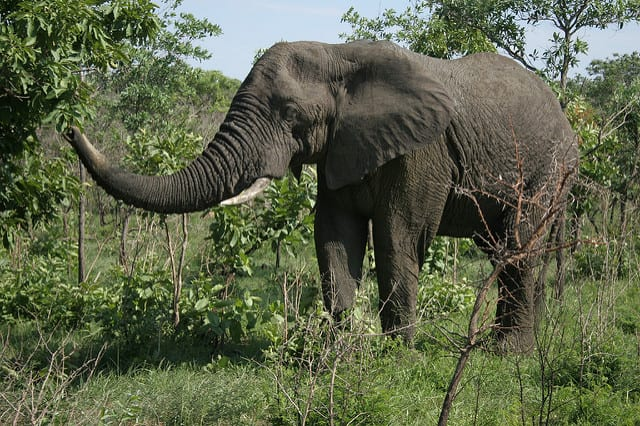
\includegraphics[width=3cm,height=4cm]{elephant.jpg}};
    \node (dummy1)  [process=white, below=of anchor, yshift=1cm]  {\textbf{X Image}};
    \node (search)  [process=gray, right=of detect2]  {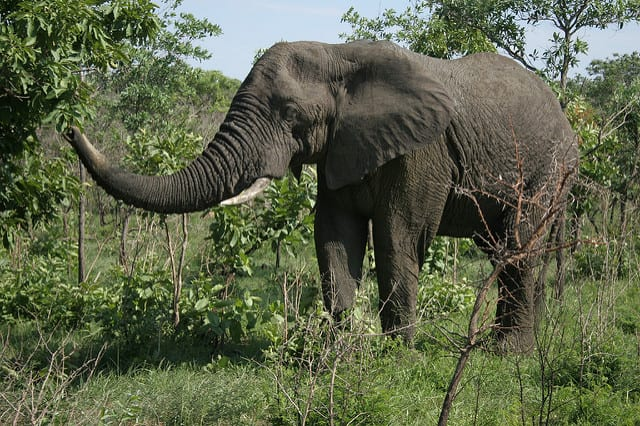
\includegraphics[width=3cm,height=4cm]{elephant.jpg}};
    \node (dummy2)  [process=white, below=of search, yshift=1cm]  {\textbf{Y Image}};

    \node (vggf1)        [process=cyan, below=of dummy1] {\textbf{some text}};
    \node (vggf2)        [process=cyan, below=of dummy2] {\textbf{some text}};

    \matrix (A) [matrix of nodes, below=of vggf1, nodes in empty cells, nodes={draw, fill=yellow!20!white, minimum size=6mm,line width=1.5pt},
    column sep=-\pgflinewidth]{ &  &  & \ldots &  \\};
    \node (dummy3)  [process=white, below=of A, yshift=1cm]  {\textbf{some text}};
    \matrix (B) [matrix of nodes, below=of vggf2, nodes in empty cells, nodes={draw, fill=yellow!20!white, minimum size=6mm,line width=1.5pt},
    column sep=-\pgflinewidth]{ &  &  & \ldots &  \\};
    \node (dummy4)  [process=white, below=of B, yshift=1cm, fill=green!20!white]  {\textbf{some text}};

    \scoped[on background layer]
    \node (instructions) [block=gray, inner xsep=0.05cm, fill=green!20!white,
          fit=(vggf2) (B) (dummy4)]   {};

    \node (cosine)    [decision=gray, below right=of A, xshift=-0.6cm, yshift=-1cm] {some text};
    \node (found)  [startstop, below=of cosine] {some text};

    \draw [solid,line width=1mm,->]
                     (dummy1)   edge (vggf1)
                     (dummy2)  edge (vggf2)
                     (vggf1)  edge (A)
                     (vggf2)  edge (B)
                     (cosine) edge node[anchor=east] {some text} (found);

    \draw[solid,line width=1mm,->] (dummy3.south)   |- node[anchor=north] {some text} (cosine.west);
    \draw[solid,line width=1mm,->] (instructions.south)   |- node[anchor=north] {some text} (cosine.east);
    \draw[solid,line width=1mm,->] (instructions.south)   |- node[anchor=west, yshift=0.5cm] {some text} (cosine.east);

    \end{tikzpicture}
\caption{Place your caption here}
\label{fig1}
\end{figure}

\end{document}
